\documentclass{sig-alternate-2013}
\pdfminorversion=4

\newfont{\mycrnotice}{ptmr8t at 7pt}
\newfont{\myconfname}{ptmri8t at 7pt}
\let\crnotice\mycrnotice%
\let\confname\myconfname%
\permission{Permission to make digital or hard copies of all or part of this work for personal or classroom use is granted without fee provided that copies are not made or distributed for profit or commercial advantage and that copies bear this notice and the full citation on the first page. Copyrights for components of this work owned by others than the author(s) must be honored. Abstracting with credit is permitted. To copy otherwise, or republish, to post on servers or to redistribute to lists, requires prior specific permission and/or a fee. Request permissions from permissions@acm.org.}
\conferenceinfo{SIGMOD'14,}{June 22--27, 2014, Snowbird, UT, USA. \\
{\mycrnotice{Copyright is held by the owner/author(s). Publication rights licensed to ACM.}}}
\copyrightetc{ACM \the\acmcopyr}
\crdata{978-1-4503-2376-5/14/06\ ...\$15.00.\\
\href{http://dx.doi.org/10.1145/2588555.2595631}{http://dx.doi.org/10.1145/2588555.2595631}}
\clubpenalty=10000
\widowpenalty = 10000

\usepackage{graphicx}
\usepackage{balance}
\usepackage{fontspec}
\setmainfont[Ligatures={TeX}]{Times}
\usepackage{hyperref}
\graphicspath{{figures/}}
\usepackage{enumitem}

\hyphenation{metamarkets nelson cheddar}

\begin{document}

% ****************** TITLE ****************************************

\title{Druid}
\subtitle{A Real-time Analytical Data Store}

% ****************** AUTHORS **************************************

\numberofauthors{6}
\author{
\alignauthor Fangjin Yang\\
  \affaddr{Metamarkets Group, Inc.}\\
  % \affaddr{625 2nd St Suite 230}\\
  % \affaddr{San Francisco, CA 94107}\\
  \email{fangjin@metamarkets.com}
\alignauthor Eric Tschetter\\
  \email{echeddar@gmail.com}
\alignauthor Xavier Léauté\\
  \affaddr{Metamarkets Group, Inc.}\\
  \email{xavier@metamarkets.com}
\and
\alignauthor Nelson Ray\\
  \email{ncray86@gmail.com}
\alignauthor Gian Merlino\\
  \affaddr{Metamarkets Group, Inc.}\\
  \email{gian@metamarkets.com}
\alignauthor Deep Ganguli\\
  \affaddr{Metamarkets Group, Inc.}\\
  \email{deep@metamarkets.com}
}
\date{21 March 2013}

% ****************** AUTHORS **************************************

\maketitle

\begin{abstract}
Druid is an open source\footnote{\href{http://druid.io/}{http://druid.io/} \href{https://github.com/apache/incubator-druid}{https://github.com/apache/incubator-druid}}
data store designed for real-time exploratory analytics on large data sets.
The system combines a column-oriented storage layout, a distributed,
shared-nothing architecture, and an advanced indexing structure to allow for
the arbitrary exploration of billion-row tables with sub-second latencies. In
this paper, we describe Druid's architecture, and detail how it supports fast
aggregations, flexible filters, and low latency data ingestion.
\end{abstract}

% A category with the (minimum) three required fields
\category{H.2.4}{Database Management}{Systems}[Distributed databases]
% \category{D.2.8}{Software Engineering}{Metrics}[complexity measures, performance measures]
\keywords{distributed; real-time; fault-tolerant; highly available; open source; analytics; column-oriented; OLAP}


\section{Introduction}
In recent years, the proliferation of internet technology has
created a surge in machine-generated events. Individually, these
events contain minimal useful information and are of low value. Given the
time and resources required to extract meaning from large collections of
events, many companies were willing to discard this data instead. Although
infrastructure has been built to handle event-based data (e.g. IBM's
Netezza\cite{singh2011introduction}, HP's Vertica\cite{bear2012vertica}, and EMC's
Greenplum\cite{miner2012unified}), they are largely sold at high price points
and are only targeted towards those companies who can afford the offering.

A few years ago, Google introduced MapReduce \cite{dean2008mapreduce} as their
mechanism of leveraging commodity hardware to index the internet and analyze
logs. The Hadoop \cite{shvachko2010hadoop} project soon followed and was
largely patterned after the insights that came out of the original MapReduce
paper. Hadoop is currently deployed in many organizations to store and analyze
large amounts of log data. Hadoop has contributed much to helping companies
convert their low-value event streams into high-value aggregates for a variety
of applications such as business intelligence and A-B testing.

As with many great systems, Hadoop has opened our eyes to a new space of
problems. Specifically, Hadoop excels at storing and providing access to large
amounts of data, however, it does not make any performance guarantees around
how quickly that data can be accessed. Furthermore, although Hadoop is a
highly available system, performance degrades under heavy concurrent load.
Lastly, while Hadoop works well for storing data, it is not optimized for
ingesting data and making that data immediately readable.

Early on in the development of the Metamarkets product, we ran into each of
these issues and came to the realization that Hadoop is a great back-office,
batch processing, and data warehousing system. However, as a company that has
product-level guarantees around query performance and data availability in a
highly concurrent environment (1000+ users), Hadoop wasn't going to meet our
needs. We explored different solutions in the space, and after
trying both Relational Database Management Systems and NoSQL architectures, we
came to the conclusion that there was nothing in the open source world that
could be fully leveraged for our requirements. We ended up creating Druid, an
open source, distributed, column-oriented, real-time analytical data store. In
many ways, Druid shares similarities with other OLAP systems
\cite{oehler2012ibm, schrader2009oracle, lachev2005applied},
interactive query systems \cite{melnik2010dremel}, main-memory databases
\cite{farber2012sap}, as well as widely known distributed data stores
\cite{chang2008bigtable, decandia2007dynamo, lakshman2010cassandra}. The
distribution and query model also borrow ideas from current generation search
infrastructure \cite{linkedin2013senseidb, apache2013solr,
banon2013elasticsearch}.

This paper describes the architecture of Druid, explores the various design
decisions made in creating an always-on production system that powers a hosted
service, and attempts to help inform anyone who faces a similar problem about a
potential method of solving it. Druid is deployed in production at several
technology
companies\footnote{\href{http://druid.org/apache/druid.html}{http://druid.org/apache/druid.html}}.
The structure of the paper is as follows: we first describe the problem in
Section \ref{sec:problem-definition}. Next, we detail system architecture from
the point of view of how data flows through the system in Section
\ref{sec:architecture}. We then discuss how and why data gets converted into a
binary format in Section \ref{sec:storage-format}. We briefly describe the
query API in Section \ref{sec:query-api} and present performance results
in Section \ref{sec:benchmarks}. Lastly, we leave off with our lessons from
running Druid in production in Section \ref{sec:production}, and related work
in Section \ref{sec:related}.

\section{Problem Definition}
\label{sec:problem-definition}

\begin{table*}
  \centering
  \begin{tabular}{| l | l | l | l | l | l | l | l |}
    \hline
    \textbf{Timestamp} & \textbf{Page} & \textbf{Username} & \textbf{Gender} & \textbf{City} & \textbf{Characters Added} & \textbf{Characters Removed} \\ \hline
    2011-01-01T01:00:00Z & Justin Bieber & Boxer & Male & San Francisco & 1800 & 25 \\ \hline
    2011-01-01T01:00:00Z & Justin Bieber & Reach & Male & Waterloo & 2912 & 42 \\ \hline
    2011-01-01T02:00:00Z & Ke\$ha & Helz & Male & Calgary & 1953 & 17 \\ \hline
    2011-01-01T02:00:00Z & Ke\$ha & Xeno & Male & Taiyuan & 3194 & 170 \\ \hline
  \end{tabular}
  \caption{Sample Druid data for edits that have occurred on Wikipedia.}
  \label{tab:sample_data}
\end{table*}


Druid was originally designed to solve problems around ingesting and exploring
large quantities of transactional events (log data). This form of timeseries
data is commonly found in OLAP workflows and the nature of the data tends to be
very append heavy. For example, consider the data shown in
Table~\ref{tab:sample_data}. Table~\ref{tab:sample_data} contains data for
edits that have occurred on Wikipedia. Each time a user edits a page in
Wikipedia, an event is generated that contains metadata about the edit. This
metadata is comprised of 3 distinct components. First, there is a timestamp
column indicating when the edit was made. Next, there are a set dimension
columns indicating various attributes about the edit such as the page that was
edited, the user who made the edit, and the location of the user. Finally,
there are a set of metric columns that contain values (usually numeric) that
can be aggregated, such as the number of characters added or removed in an
edit.

Our goal is to rapidly compute drill-downs and aggregates over this data. We
want to answer questions like “How many edits were made on the page Justin
Bieber from males in San Francisco?” and “What is the average number of
characters that were added by people from Calgary over the span of a month?”. We also
want queries over any arbitrary combination of dimensions to return with
sub-second latencies.

The need for Druid was facilitated by the fact that existing open source
Relational Database Management Systems (RDBMS) and NoSQL key/value stores were
unable to provide a low latency data ingestion and query platform for
interactive applications \cite{tschetter2011druid}. In the early days of
Metamarkets, we were focused on building a hosted dashboard that would allow
users to arbitrarily explore and visualize event streams. The data store
powering the dashboard needed to return queries fast enough that the data
visualizations built on top of it could provide users with an interactive
experience.

In addition to the query latency needs, the system had to be multi-tenant and
highly available. The Metamarkets product is used in a highly concurrent
environment. Downtime is costly and many businesses cannot afford to wait if a
system is unavailable in the face of software upgrades or network failure.
Downtime for startups, who often lack proper internal operations management, can
determine business success or failure.

Finally, another challenge that Metamarkets faced in its early days was to
allow users and alerting systems to be able to make business decisions in
``real-time". The time from when an event is created to when that event is
queryable determines how fast interested parties are able to react to
potentially catastrophic situations in their systems. Popular open source data
warehousing systems such as Hadoop were unable to provide the sub-second data
ingestion latencies we required.

The problems of data exploration, ingestion, and availability span multiple
industries. Since Druid was open sourced in October 2012, it been deployed as a
video, network monitoring, operations monitoring, and online advertising
analytics platform at multiple companies.

\section{Architecture}
\label{sec:architecture}
A Druid cluster consists of different types of nodes and each node type is
designed to perform a specific set of things. We believe this design separates
concerns and simplifies the complexity of the overall system. The different
node types operate fairly independent of each other and there is minimal
interaction among them. Hence, intra-cluster communication failures have
minimal impact on data availability.

To solve complex data analysis problems, the different node types come together
to form a fully working system. The name Druid comes from the Druid class in
many role-playing games: it is a shape-shifter, capable of taking on many
different forms to fulfill various different roles in a group. The composition
of and flow of data in a Druid cluster are shown in Figure~\ref{fig:cluster}.

\begin{figure*}
\centering
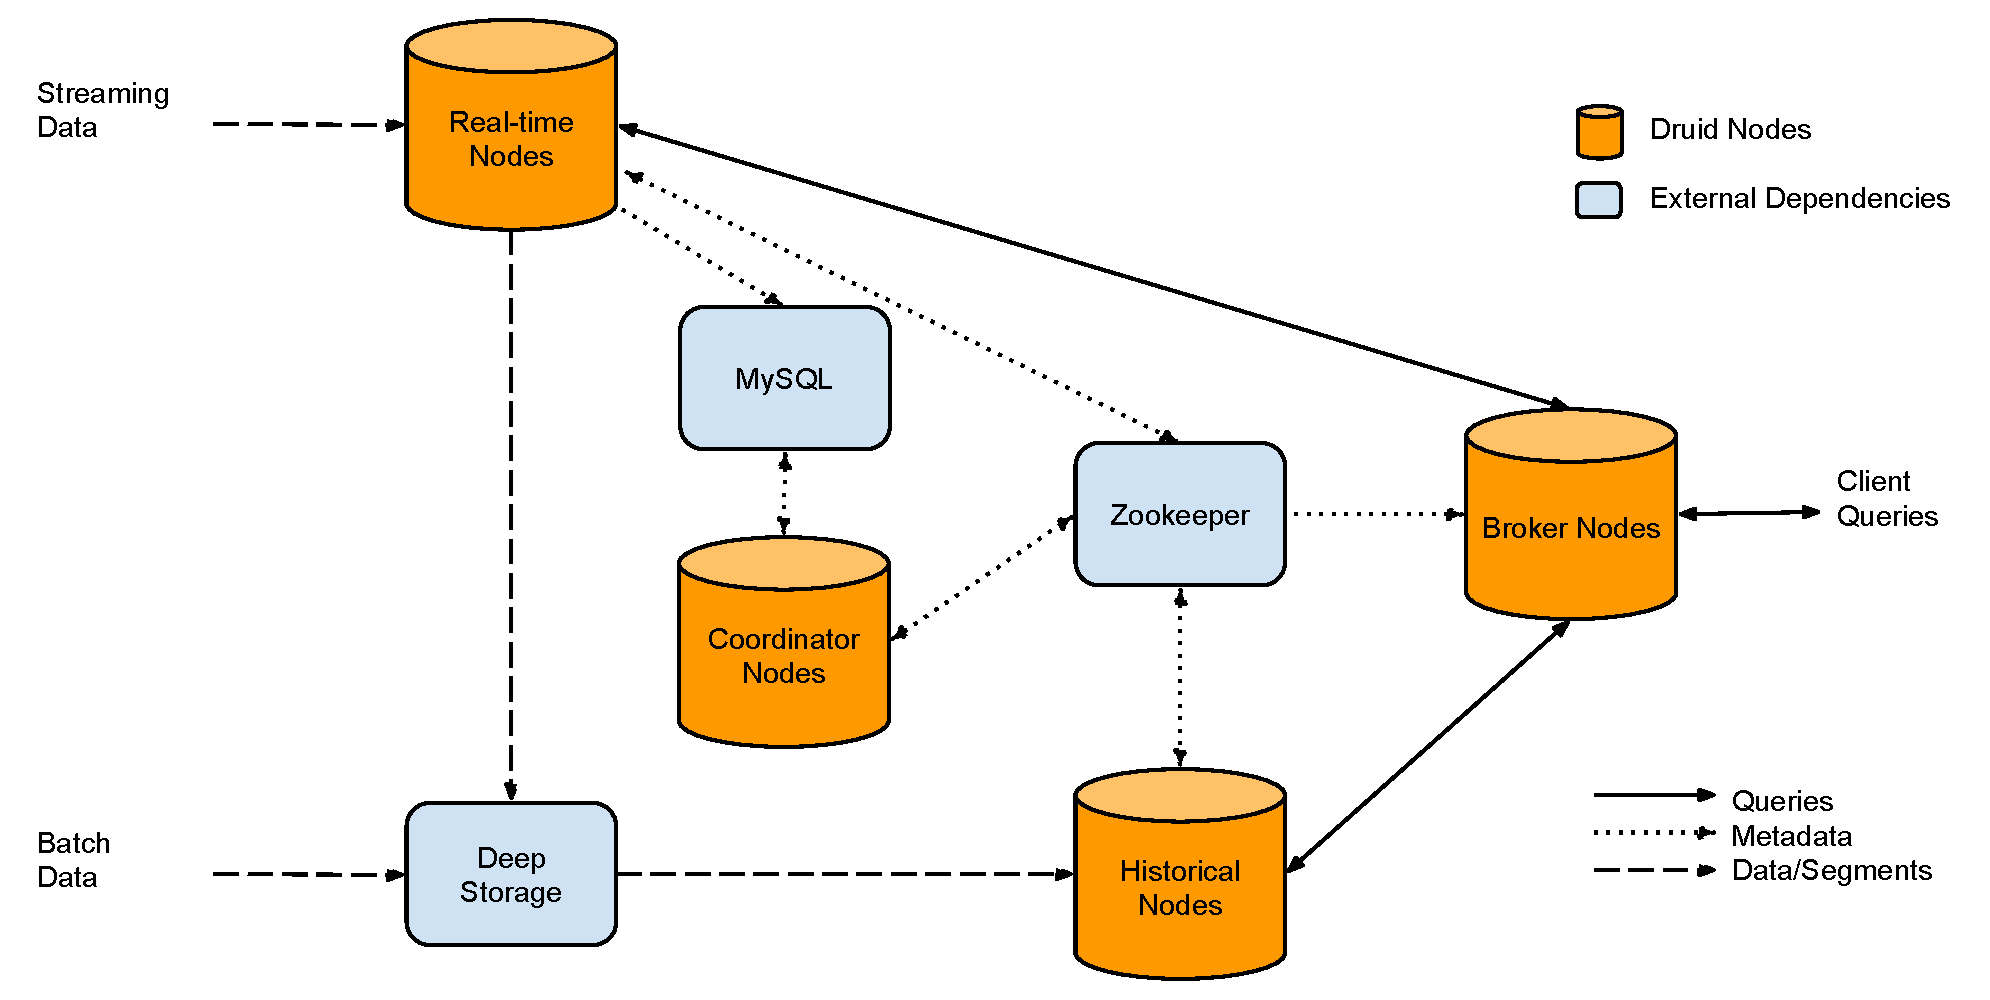
\includegraphics[width = 4.5in]{cluster}
\caption{An overview of a Druid cluster and the flow of data through the cluster.}
\label{fig:cluster}
\end{figure*}

\subsection{Real-time Nodes}
\label{sec:realtime}
Real-time nodes encapsulate the functionality to ingest and query event
streams. Events indexed via these nodes are immediately available for querying.
The nodes are only concerned with events for some small time range and
periodically hand off immutable batches of events they have collected over this
small time range to other nodes in the Druid cluster that are specialized in
dealing with batches of immutable events. Real-time nodes leverage ZooKeeper
\cite{hunt2010zookeeper} for coordination with the rest of the Druid cluster.
The nodes announce their online state and the data they serve in
ZooKeeper.

Real-time nodes maintain an in-memory index buffer for all incoming events.
These indexes are incrementally populated as events are ingested and the
indexes are also directly queryable. Druid behaves as a row store
for queries on events that exist in this JVM heap-based buffer. To avoid heap
overflow problems, real-time nodes persist their in-memory indexes to disk
either periodically or after some maximum row limit is reached. This persist
process converts data stored in the in-memory buffer to a column oriented
storage format described in Section \ref{sec:storage-format}. Each persisted
index is immutable and real-time nodes load persisted indexes into off-heap
memory such that they can still be queried. This process is described in detail
in \cite{o1996log} and is illustrated in Figure~\ref{fig:realtime_flow}.

\begin{figure}
\centering
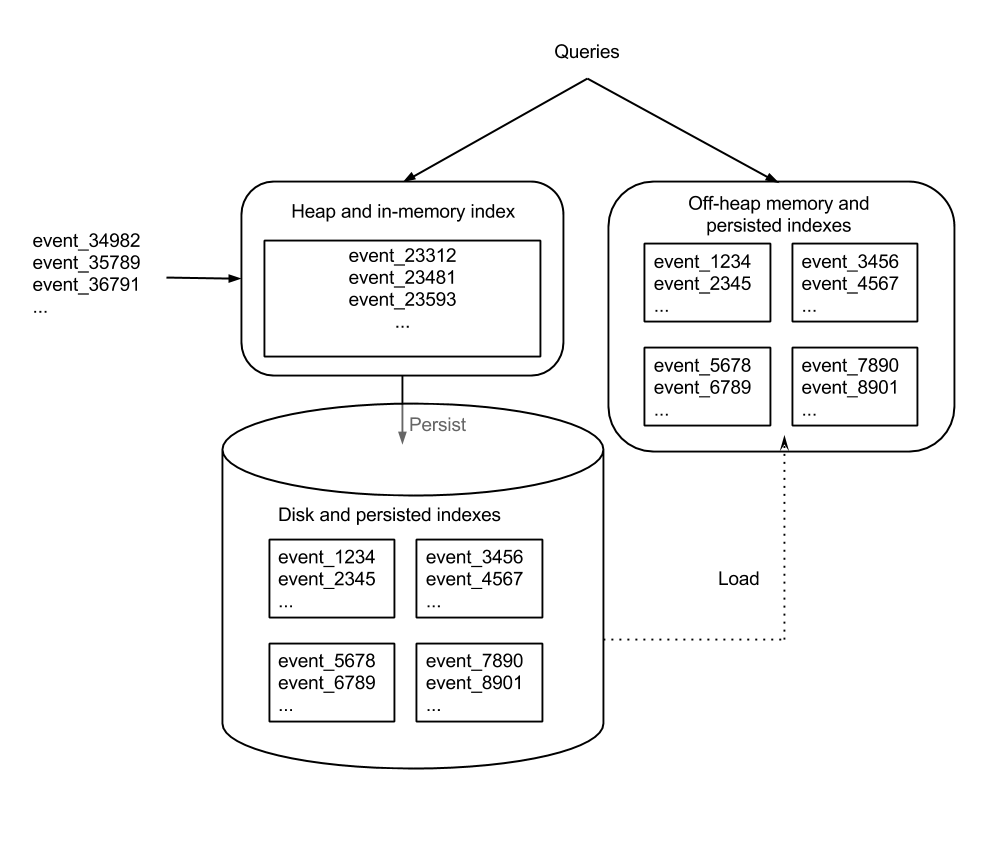
\includegraphics[width = 2.6in]{realtime_flow}
\caption{Real-time nodes buffer events to an in-memory index, which is
regularly persisted to disk. On a periodic basis, persisted indexes are then merged
together before getting handed off.
Queries will hit both the in-memory and persisted indexes.
}
\label{fig:realtime_flow}
\end{figure}

On a periodic basis, each real-time node will schedule a background task that
searches for all locally persisted indexes. The task merges these indexes
together and builds an immutable block of data that contains all the events
that have been ingested by a real-time node for some span of time. We refer to this
block of data as a ``segment". During the handoff stage, a real-time node
uploads this segment to a permanent backup storage, typically a distributed
file system such as S3 \cite{decandia2007dynamo} or HDFS
\cite{shvachko2010hadoop}, which Druid refers to as ``deep storage". The ingest,
persist, merge, and handoff steps are fluid; there is no data loss during any
of the processes.

Figure~\ref{fig:realtime_timeline} illustrates the operations of a real-time
node. The node starts at 13:37 and will only accept events for the current hour
or the next hour. When events are ingested, the node announces that it is
serving a segment of data for an interval from 13:00 to 14:00. Every 10
minutes (the persist period is configurable), the node will flush and persist
its in-memory buffer to disk. Near the end of the hour, the node will likely
see events for 14:00 to 15:00. When this occurs, the node prepares to serve
data for the next hour and creates a new in-memory index. The node then
announces that it is also serving a segment from 14:00 to 15:00. The node does
not immediately merge persisted indexes from 13:00 to 14:00, instead it waits
for a configurable window period for straggling events from 13:00 to 14:00 to
arrive. This window period minimizes the risk of data loss from delays in event
delivery. At the end of the window period, the node merges all persisted
indexes from 13:00 to 14:00 into a single immutable segment and hands the
segment off. Once this segment is loaded and queryable somewhere else in the
Druid cluster, the real-time node flushes all information about the data it
collected for 13:00 to 14:00 and unannounces it is serving this data.

\begin{figure*}
\centering

\includegraphics[width = 4.5in]{realtime_timeline}
\caption{The node starts, ingests data, persists, and periodically hands data
off. This process repeats indefinitely. The time periods between different
real-time node operations are configurable.}
\label{fig:realtime_timeline}
\end{figure*}

\subsubsection{Availability and Scalability}
Real-time nodes are a consumer of data and require a corresponding producer to
provide the data stream. Commonly, for data durability purposes, a message
bus such as Kafka \cite{kreps2011kafka} sits between the producer and the
real-time node as shown in Figure~\ref{fig:realtime_pipeline}. Real-time nodes
ingest data by reading events from the message bus. The time from event
creation to event consumption is ordinarily on the order of hundreds of
milliseconds.

\begin{figure}
\centering
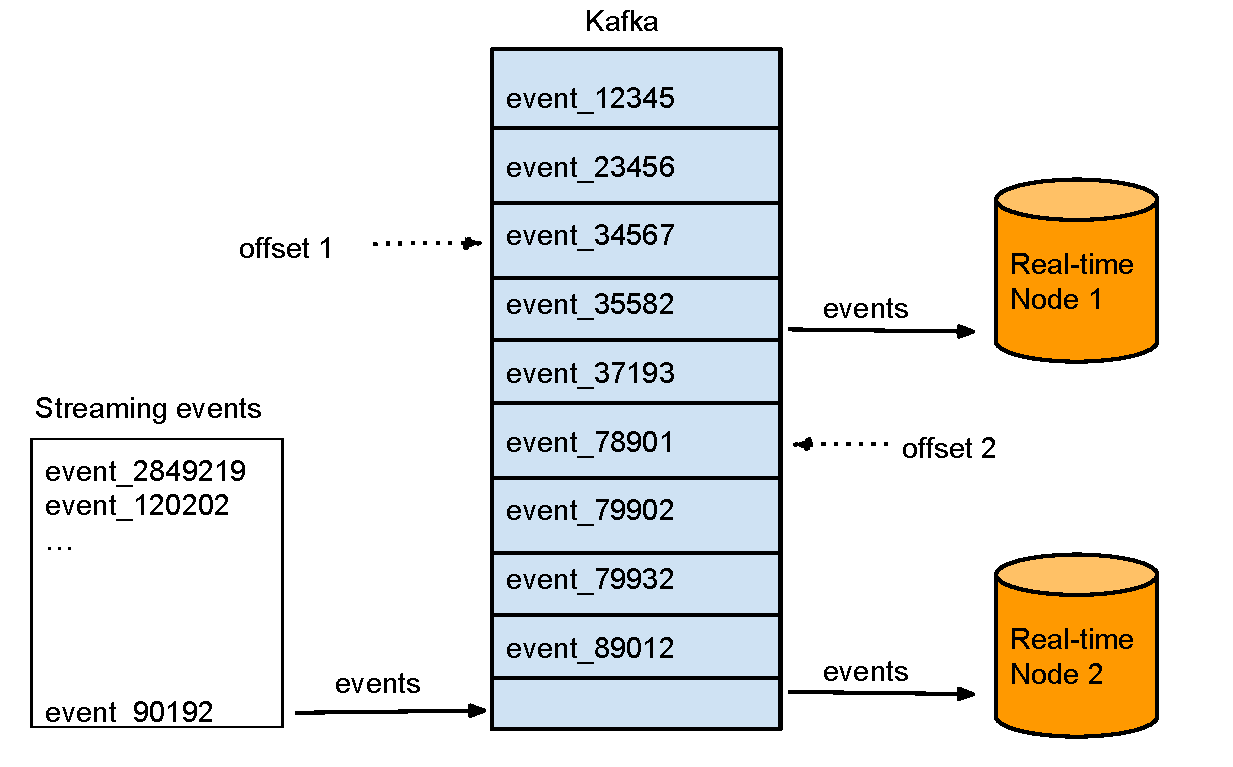
\includegraphics[width = 2.8in]{realtime_pipeline}
\caption{Multiple real-time nodes can read from the same message bus. Each node maintains its own offset.}
\label{fig:realtime_pipeline}
\end{figure}

The purpose of the message bus in Figure~\ref{fig:realtime_pipeline} is
two-fold. First, the message bus acts as a buffer for incoming events. A
message bus such as Kafka maintains positional offsets indicating how far a
consumer (a real-time node) has read in an event stream. Consumers can
programmatically update these offsets. Real-time nodes update this offset each
time they persist their in-memory buffers to disk. In a fail and recover
scenario, if a node has not lost disk, it can reload all persisted indexes from
disk and continue reading events from the last offset it committed. Ingesting
events from a recently committed offset greatly reduces a node's recovery time.
In practice, we see nodes recover from such failure scenarios in a
few seconds.

The second purpose of the message bus is to act as a single endpoint from which
multiple real-time nodes can read events. Multiple real-time nodes can ingest
the same set of events from the bus, creating a replication of events. In a
scenario where a node completely fails and loses disk, replicated streams
ensure that no data is lost. A single ingestion endpoint also allows for data
streams to be partitioned such that multiple real-time nodes each ingest a
portion of a stream. This allows additional real-time nodes to be seamlessly
added. In practice, this model has allowed one of the largest production Druid
clusters to be able to consume raw data at approximately 500 MB/s (150,000
events/s or 2 TB/hour).

\subsection{Historical Nodes}
Historical nodes encapsulate the functionality to load and serve the immutable
blocks of data (segments) created by real-time nodes. In many real-world
workflows, most of the data loaded in a Druid cluster is immutable and hence,
historical nodes are typically the main workers of a Druid cluster. Historical
nodes follow a shared-nothing architecture and there is no single point of
contention among the nodes. The nodes have no knowledge of one another and are
operationally simple; they only know how to load, drop, and serve immutable
segments.

Similar to real-time nodes, historical nodes announce their online state and
the data they are serving in ZooKeeper. Instructions to load and drop segments
are sent over ZooKeeper and contain information about where the segment is
located in deep storage and how to decompress and process the segment. Before
a historical node downloads a particular segment from deep storage, it first
checks a local cache that maintains information about what segments already
exist on the node. If information about a segment is not present in the cache,
the historical node will proceed to download the segment from deep storage.
This process is shown in Figure~\ref{fig:historical_download}. Once processing
is complete, the segment is announced in ZooKeeper. At this point, the segment
is queryable. The local cache also allows for historical nodes to be quickly
updated and restarted. On startup, the node examines its cache and immediately
serves whatever data it finds.

\begin{figure}
\centering
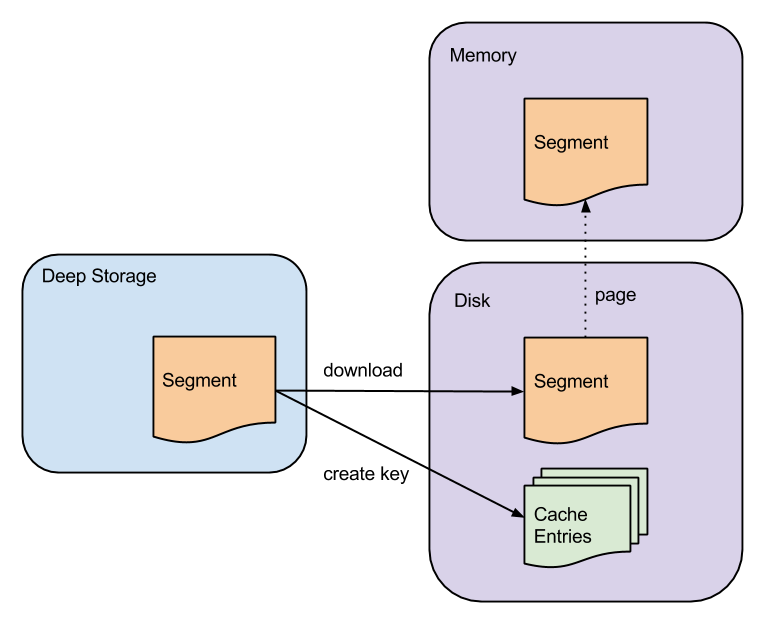
\includegraphics[width = 2.6in]{historical_download}
\caption{Historical nodes download immutable segments from deep storage. Segments must be loaded in memory before they can be queried.}
\label{fig:historical_download}
\end{figure}

Historical nodes can support read consistency because they only deal with
immutable data. Immutable data blocks also enable a simple parallelization
model: historical nodes can concurrently scan and aggregate immutable blocks
without blocking.

\subsubsection{Tiers}
\label{sec:tiers}
Historical nodes can be grouped in different tiers, where all nodes in a
given tier are identically configured. Different performance and
fault-tolerance parameters can be set for each tier. The purpose of
tiered nodes is to enable higher or lower priority segments to be
distributed according to their importance. For example, it is possible
to spin up a “hot” tier of historical nodes that have a high number of
cores and large memory capacity. The “hot” cluster can be configured to
download more frequently accessed data. A parallel “cold” cluster
can also be created with much less powerful backing hardware. The
“cold” cluster would only contain less frequently accessed segments.

\subsubsection{Availability}
Historical nodes depend on ZooKeeper for segment load and unload instructions.
Should ZooKeeper become unavailable, historical nodes are no longer able to serve
new data or drop outdated data, however, because the queries are served over
HTTP, historical nodes are still able to respond to query requests for
the data they are currently serving. This means that ZooKeeper outages do not
impact current data availability on historical nodes.

\subsection{Broker Nodes}
Broker nodes act as query routers to historical and real-time nodes. They
understand the metadata published in ZooKeeper about what segments are
queryable and where those segments are located. Broker nodes route incoming queries
such that the queries hit the right historical or real-time nodes. Broker nodes
also merge partial results from historical and real-time nodes before returning
a final consolidated result to the caller.

\subsubsection{Caching}
\label{sec:caching}
Broker nodes contain a cache with a LRU \cite{o1993lru, kim2001lrfu}
invalidation strategy. The cache can use local heap memory or an external
distributed key/value store such as Memcached
\cite{fitzpatrick2004distributed}. Each time a broker node receives a query, it
first maps the query to a set of segments. Results for certain segments may
already exist in the cache and there is no need to recompute them. For any
results that do not exist in the cache, the broker node will forward the query
to the correct historical and real-time nodes. Once historical nodes return
their results, the broker will cache these results on a per-segment basis for
future use. This process is illustrated in Figure~\ref{fig:caching}. Real-time
data is never cached and hence requests for real-time data will always be
forwarded to real-time nodes. Real-time data is perpetually changing and
caching the results is unreliable.

\begin{figure*}
\centering

\includegraphics[width = 4.5in]{caching}
\caption{Results are cached per-segment. Queries combine cached results with results computed on historical and real-time nodes.}
\label{fig:caching}
\end{figure*}

The cache also acts as an additional level of data durability. In the event
that all historical nodes fail, it is still possible to query results if those
results already exist in the cache.

\subsubsection{Availability}
In the event of a total ZooKeeper outage, data is still queryable. If broker
nodes are unable to communicate to ZooKeeper, they use their last known view of
the cluster and continue to forward queries to real-time and historical nodes.
Broker nodes make the assumption that the structure of the cluster is the same
as it was before the outage. In practice, this availability model has allowed
our Druid cluster to continue serving queries for a significant period of time while we
diagnosed ZooKeeper outages.

\subsection{Coordinator Nodes}
Druid coordinator nodes are primarily in charge of data management and
distribution on historical nodes. The coordinator nodes tell historical nodes
to load new data, drop outdated data, replicate data, and move data to load
balance. Druid uses a multi-version concurrency control swapping protocol for
managing immutable segments in order to maintain stable views. If any
immutable segment contains data that is wholly obsoleted by newer segments, the
outdated segment is dropped from the cluster. Coordinator nodes undergo a
leader-election process that determines a single node that runs the coordinator
functionality. The remaining coordinator nodes act as redundant backups.

A coordinator node runs periodically to determine the current state of the
cluster. It makes decisions by comparing the expected state of the cluster with
the actual state of the cluster at the time of the run. As with all Druid
nodes, coordinator nodes maintain a ZooKeeper connection for current cluster
information. Coordinator nodes also maintain a connection to a MySQL
database that contains additional operational parameters and configurations.
One of the key pieces of information located in the MySQL database is a table
that contains a list of all segments that should be served by historical nodes.
This table can be updated by any service that creates segments, for example,
real-time nodes. The MySQL database also contains a rule table that governs how
segments are created, destroyed, and replicated in the cluster.

\subsubsection{Rules}
Rules govern how historical segments are loaded and dropped from the cluster.
Rules indicate how segments should be assigned to different historical node
tiers and how many replicates of a segment should exist in each tier. Rules may
also indicate when segments should be dropped entirely from the cluster. Rules
are usually set for a period of time. For example, a user may use rules to
load the most recent one month's worth of segments into a ``hot" cluster, the
most recent one year's worth of segments into a ``cold" cluster, and drop any
segments that are older.

The coordinator nodes load a set of rules from a rule table in the MySQL
database. Rules may be specific to a certain data source and/or a default set
of rules may be configured. The coordinator node will cycle through all available
segments and match each segment with the first rule that applies to it.

\subsubsection{Load Balancing}
In a typical production environment, queries often hit dozens or even hundreds
of segments. Since each historical node has limited resources, segments must be
distributed among the cluster to ensure that the cluster load is not too
imbalanced. Determining optimal load distribution requires some knowledge about
query patterns and speeds. Typically, queries cover recent segments spanning
contiguous time intervals for a single data source. On average, queries that
access smaller segments are faster.

These query patterns suggest replicating recent historical segments at a higher
rate, spreading out large segments that are close in time to different
historical nodes, and co-locating segments from different data sources. To
optimally distribute and balance segments among the cluster, we developed a
cost-based optimization procedure that takes into account the segment data
source, recency, and size. The exact details of the algorithm are beyond the
scope of this paper and may be discussed in future literature.

\subsubsection{Replication}
Coordinator nodes may tell different historical nodes to load a copy of the
same segment. The number of replicates in each tier of the historical compute
cluster is fully configurable. Setups that require high levels of fault
tolerance can be configured to have a high number of replicas. Replicated
segments are treated the same as the originals and follow the same load
distribution algorithm. By replicating segments, single historical node
failures are transparent in the Druid cluster. We use this property for
software upgrades. We can seamlessly take a historical node offline, update it,
bring it back up, and repeat the process for every historical node in a
cluster. Over the last two years, we have never taken downtime in our Druid
cluster for software upgrades.

\subsubsection{Availability}
Druid coordinator nodes have ZooKeeper and MySQL as external dependencies.
Coordinator nodes rely on ZooKeeper to determine what historical nodes already
exist in the cluster. If ZooKeeper becomes unavailable, the coordinator will no
longer be able to send instructions to assign, balance, and drop segments.
However, these operations do not affect data availability at all.

The design principle for responding to MySQL and ZooKeeper failures is the
same: if an external dependency responsible for coordination fails, the cluster
maintains the status quo. Druid uses MySQL to store operational management
information and segment metadata information about what segments should exist
in the cluster. If MySQL goes down, this information becomes unavailable to
coordinator nodes. However, this does not mean data itself is unavailable. If
coordinator nodes cannot communicate to MySQL, they will cease to assign new
segments and drop outdated ones. Broker, historical, and real-time nodes are still
queryable during MySQL outages.

\section{Storage Format}
\label{sec:storage-format}
Data tables in Druid (called \emph{data sources}) are collections of
timestamped events and partitioned into a set of segments, where each segment
is typically 5--10 million rows. Formally, we define a segment as a collection
of rows of data that span some period of time. Segments represent the
fundamental storage unit in Druid and replication and distribution are done at
a segment level.

Druid always requires a timestamp column as a method of simplifying data
distribution policies, data retention policies, and first-level query pruning.
Druid partitions its data sources into well-defined time intervals, typically
an hour or a day, and may further partition on values from other columns to
achieve the desired segment size. The time granularity
to partition segments is a function of data volume and time range. A data set
with timestamps spread over a year is better partitioned by day, and a data set
with timestamps spread over a day is better partitioned by hour.

Segments are uniquely identified by a data source identifer, the time interval
of the data, and a version string that increases whenever a new segment is
created. The version string indicates the freshness of segment data; segments
with later versions have newer views of data (over some time range) than
segments with older versions. This segment metadata is used by the system for
concurrency control; read operations always access data in a particular time
range from the segments with the latest version identifiers for that time
range.

Druid segments are stored in a column orientation. Given that Druid is best
used for aggregating event streams (all data going into Druid must have a
timestamp), the advantages of storing aggregate information as columns rather than
rows are well documented \cite{abadi2008column}. Column storage allows for more
efficient CPU usage as only what is needed is actually loaded and scanned. In a
row oriented data store, all columns associated with a row must be scanned as
part of an aggregation. The additional scan time can introduce signficant performance
degradations \cite{abadi2008column}.

Druid has multiple column types to represent various data formats. Depending on
the column type, different compression methods are used to reduce the cost of
storing a column in memory and on disk. In the example given in
Table~\ref{tab:sample_data}, the page, user, gender, and city columns only
contain strings. Storing strings directly is unnecessarily costly and string
columns can be dictionary encoded instead. Dictionary encoding is a common
method to compress data and has been used in other data stores such as
PowerDrill \cite{hall2012processing}. In the example in
Table~\ref{tab:sample_data}, we can map each page to a unique integer
identifier.
{\small\begin{verbatim}
Justin Bieber   -> 0
Ke$ha -> 1
\end{verbatim}}
This mapping allows us to represent the page column as an integer
array where the array indices correspond to the rows of the original
data set. For the page column, we can represent the unique
pages as follows:
{\small\begin{verbatim}
[0, 0, 1, 1]
\end{verbatim}}

The resulting integer array lends itself very well to
compression methods. Generic compression algorithms on top of encodings are
extremely common in column-stores. Druid uses the LZF \cite{liblzf2013} compression
algorithm.

Similar compression methods can be applied to numeric
columns. For example, the characters added and characters removed columns in
Table~\ref{tab:sample_data} can also be expressed as individual
arrays.
{\small\begin{verbatim}
Characters Added   -> [1800, 2912, 1953, 3194]
Characters Removed -> [25, 42, 17, 170]
\end{verbatim}}
In this case, we compress the raw values as opposed to their dictionary
representations.

\subsection{Indices for Filtering Data}
In many real world OLAP workflows, queries are issued for the aggregated
results of some set of metrics where some set of dimension specifications are
met. An example query is: ``How many Wikipedia edits were done by users in
San Francisco who are also male?" This query is filtering the Wikipedia data
set in Table~\ref{tab:sample_data} based on a Boolean expression of dimension
values. In many real world data sets, dimension columns contain strings and
metric columns contain numeric values. Druid creates additional lookup
indices for string columns such that only those rows that pertain to a
particular query filter are ever scanned.

Let us consider the page column in
Table~\ref{tab:sample_data}. For each unique page in
Table~\ref{tab:sample_data}, we can form some representation
indicating in which table rows a particular page is seen. We can
store this information in a binary array where the array indices
represent our rows. If a particular page is seen in a certain
row, that array index is marked as \texttt{1}. For example:
{\small\begin{verbatim}
Justin Bieber -> rows [0, 1] -> [1][1][0][0]
Ke$ha         -> rows [2, 3] -> [0][0][1][1]
\end{verbatim}}

\texttt{Justin Bieber} is seen in rows \texttt{0} and \texttt{1}. This mapping of column values
to row indices forms an inverted index \cite{tomasic1993performance}. To know which
rows contain {\ttfamily Justin Bieber} or {\ttfamily Ke\$ha}, we can \texttt{OR} together
the two arrays.
{\small\begin{verbatim}
[0][1][0][1] OR [1][0][1][0] = [1][1][1][1]
\end{verbatim}}

\begin{figure}
\centering
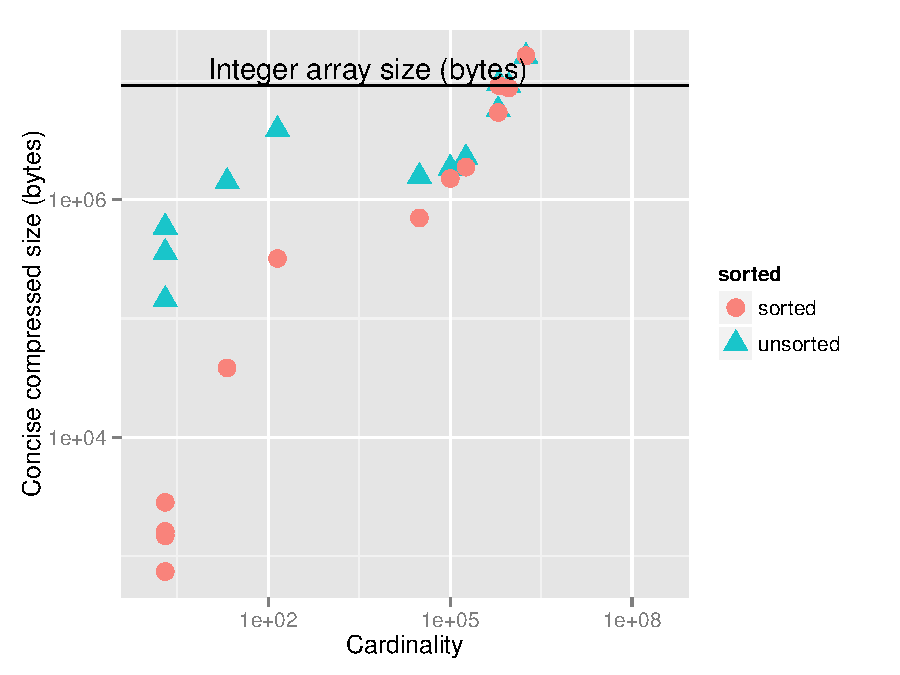
\includegraphics[width = 2.8in]{concise_plot}
\caption{Integer array size versus Concise set size.}
\label{fig:concise_plot}
\end{figure}

This approach of performing Boolean operations on large bitmap sets is commonly
used in search engines. Bitmap indices for OLAP workloads is described in
detail in \cite{o1997improved}. Bitmap compression algorithms are a
well-defined area of research \cite{antoshenkov1995byte, wu2006optimizing,
van2011memory} and often utilize run-length encoding. Druid opted to use the
Concise algorithm \cite{colantonio2010concise}. Figure~\ref{fig:concise_plot}
illustrates the number of bytes using Concise compression versus using an
integer array. The results were generated on a \texttt{cc2.8xlarge} system with
a single thread, 2G heap, 512m young gen, and a forced GC between each run. The
data set is a single day’s worth of data collected from the Twitter garden hose
\cite{twitter2013} data stream. The data set contains 2,272,295 rows and 12
dimensions of varying cardinality. As an additional comparison, we also
resorted the data set rows to maximize compression.

In the unsorted case, the total Concise size was 53,451,144 bytes and the total
integer array size was 127,248,520 bytes. Overall, Concise compressed sets are
about 42\% smaller than integer arrays. In the sorted case, the total Concise
compressed size was 43,832,884 bytes and the total integer array size was
127,248,520 bytes. What is interesting to note is that after sorting, global
compression only increased minimally.

\subsection{Storage Engine}
Druid’s persistence components allows for different storage engines to be
plugged in, similar to Dynamo \cite{decandia2007dynamo}. These storage engines
may store data in an entirely in-memory structure such as the JVM heap or in
memory-mapped structures. The ability to swap storage engines allows for Druid
to be configured depending on a particular application’s specifications. An
in-memory storage engine may be operationally more expensive than a
memory-mapped storage engine but could be a better alternative if performance
is critical. By default, a memory-mapped storage engine is used.

When using a memory-mapped storage engine, Druid relies on the operating system
to page segments in and out of memory. Given that segments can only be scanned
if they are loaded in memory, a memory-mapped storage engine allows recent
segments to retain in memory whereas segments that are never queried are paged
out. The main drawback with using the memory-mapped storage engine is when a
query requires more segments to be paged into memory than a given node has
capacity for. In this case, query performance will suffer from the cost of
paging segments in and out of memory.

\section{Query API}
\label{sec:query-api}
Druid has its own query language and accepts queries as POST requests. Broker,
historical, and real-time nodes all share the same query API.

The body of the POST request is a JSON object containing key-value pairs
specifying various query parameters. A typical query will contain the data
source name, the granularity of the result data, time range of interest, the
type of request, and the metrics to aggregate over. The result will also be a
JSON object containing the aggregated metrics over the time period.

Most query types will also support a filter set. A filter set is a Boolean
expression of dimension name and value pairs. Any number and combination of
dimensions and values may be specified. When a filter set is provided, only
the subset of the data that pertains to the filter set will be scanned. The
ability to handle complex nested filter sets is what enables Druid to drill
into data at any depth.

The exact query syntax depends on the query type and the information requested.
A sample count query over a week of data is as follows:
{\scriptsize\begin{verbatim}
{
  "queryType"    : "timeseries",
  "dataSource"   : "wikipedia",
  "intervals"    : "2013-01-01/2013-01-08",
  "filter"       : {
                     "type" : "selector",
                     "dimension" : "page",
                     "value" : "Ke$ha"
                   },
  "granularity"  : "day",
  "aggregations" : [{"type":"count", "name":"rows"}]
}
\end{verbatim}}
The query shown above will return a count of the number of rows in the Wikipedia data source
from 2013-01-01 to 2013-01-08, filtered for only those rows where the value of the ``page" dimension is
equal to ``Ke\$ha". The results will be bucketed by day and will be a JSON array of the following form:
{\scriptsize\begin{verbatim}
[ {
    "timestamp": "2012-01-01T00:00:00.000Z",
    "result": {"rows":393298}
  },
  {
    "timestamp": "2012-01-02T00:00:00.000Z",
    "result": {"rows":382932}
  },
  ...
  {
    "timestamp": "2012-01-07T00:00:00.000Z",
    "result": {"rows": 1337}
} ]
\end{verbatim}}

Druid supports many types of aggregations including sums on floating-point and integer types,
minimums, maximums, and complex aggregations such as cardinality estimation and
approximate quantile estimation. The results of aggregations can be combined
in mathematical expressions to form other aggregations. It is beyond the scope
of this paper to fully describe the query API but more information can be found
online\footnote{\href{http://druid.io/docs/latest/Querying.html}{http://druid.io/docs/latest/Querying.html}}.

As of this writing, a join query for Druid is not yet implemented. This has
been a function of engineering resource allocation and use case decisions more
than a decision driven by technical merit. Indeed, Druid's storage format
would allow for the implementation of joins (there is no loss of fidelity for
columns included as dimensions) and the implementation of them has been a
conversation that we have every few months. To date, we have made the choice
that the implementation cost is not worth the investment for our organization.
The reasons for this decision are generally two-fold.

\begin{enumerate}
\item Scaling join queries has been, in our professional experience, a constant bottleneck of working with distributed databases.
\item The incremental gains in functionality are perceived to be of less value than the anticipated problems with managing highly concurrent, join-heavy workloads.
\end{enumerate}

A join query is essentially the merging of two or more streams of data based on
a shared set of keys. The primary high-level strategies for join queries we
are aware of are a hash-based strategy or a sorted-merge strategy. The
hash-based strategy requires that all but one data set be available as
something that looks like a hash table, a lookup operation is then performed on
this hash table for every row in the ``primary" stream. The sorted-merge
strategy assumes that each stream is sorted by the join key and thus allows for
the incremental joining of the streams. Each of these strategies, however,
requires the materialization of some number of the streams either in sorted
order or in a hash table form.

When all sides of the join are significantly large tables (> 1 billion records),
materializing the pre-join streams requires complex distributed memory
management. The complexity of the memory management is only amplified by
the fact that we are targeting highly concurrent, multitenant workloads.
This is, as far as we are aware, an active academic research
problem that we would be willing to help resolve in a scalable manner.


\section{Performance}
\label{sec:benchmarks}
Druid runs in production at several organizations, and to demonstrate its
performance, we have chosen to share some real world numbers for the main production
cluster running at Metamarkets as of early 2014. For comparison with other databases
we also include results from synthetic workloads on TPC-H data.

\subsection{Query Performance in Production}
Druid query performance can vary signficantly depending on the query
being issued. For example, sorting the values of a high cardinality dimension
based on a given metric is much more expensive than a simple count over a time
range. To showcase the average query latencies in a production Druid cluster,
we selected 8 of our most queried data sources, described in Table~\ref{tab:datasources}.

Approximately 30\% of queries are standard
aggregates involving different types of metrics and filters, 60\% of queries
are ordered group bys over one or more dimensions with aggregates, and 10\% of
queries are search queries and metadata retrieval queries. The number of
columns scanned in aggregate queries roughly follows an exponential
distribution. Queries involving a single column are very frequent, and queries
involving all columns are very rare.

\begin{table}
  \centering
  \scriptsize\begin{tabular}{| l | l | l |}
    \hline
    \textbf{Data Source} & \textbf{Dimensions} & \textbf{Metrics} \\ \hline
    \texttt{a} & 25 & 21 \\ \hline
    \texttt{b} & 30 & 26 \\ \hline
    \texttt{c} & 71 & 35 \\ \hline
    \texttt{d} & 60 & 19 \\ \hline
    \texttt{e} & 29 & 8 \\ \hline
    \texttt{f} & 30 & 16 \\ \hline
    \texttt{g} & 26 & 18 \\ \hline
    \texttt{h} & 78 & 14 \\ \hline
  \end{tabular}
  \normalsize
  \caption{Characteristics of production data sources.}
  \label{tab:datasources}
\end{table}

A few notes about our results:
\begin{itemize}[leftmargin=*,beginpenalty=5000,topsep=0pt]
\item The results are from a ``hot" tier in our production cluster. There were
approximately 50 data sources in the tier and several hundred users issuing
queries.

\item There was approximately 10.5TB of RAM available in the ``hot" tier and
approximately 10TB of segments loaded. Collectively,
there are about 50 billion Druid rows in this tier. Results for
every data source are not shown.

\item The hot tier uses Intel\textsuperscript{\textregistered} Xeon\textsuperscript{\textregistered} E5-2670 processors and consists of 1302 processing
threads and 672 total cores (hyperthreaded).

\item A memory-mapped storage engine was used (the machine was configured to
    memory map the data instead of loading it into the Java heap.)
\end{itemize}

Query latencies are shown in Figure~\ref{fig:query_latency} and the queries per
minute are shown in Figure~\ref{fig:queries_per_min}. Across all the various
data sources, average query latency is approximately 550 milliseconds, with
90\% of queries returning in less than 1 second, 95\% in under 2 seconds, and
99\% of queries returning in less than 10 seconds. Occasionally we observe
spikes in latency, as observed on February 19, where network issues on
the Memcached instances were compounded by very high query load on one of our
largest data sources.

\begin{figure}
\centering
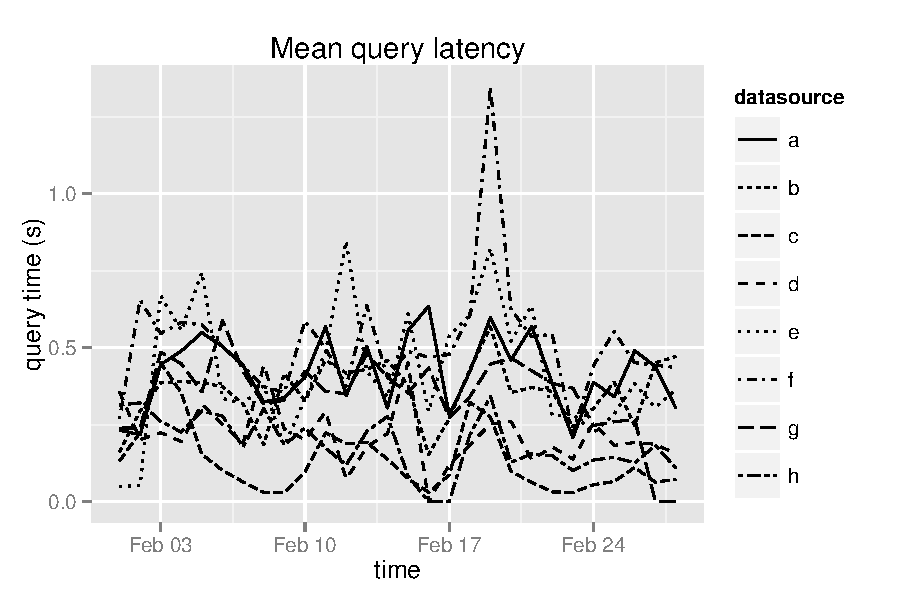
\includegraphics[width = 2.3in]{avg_query_latency}
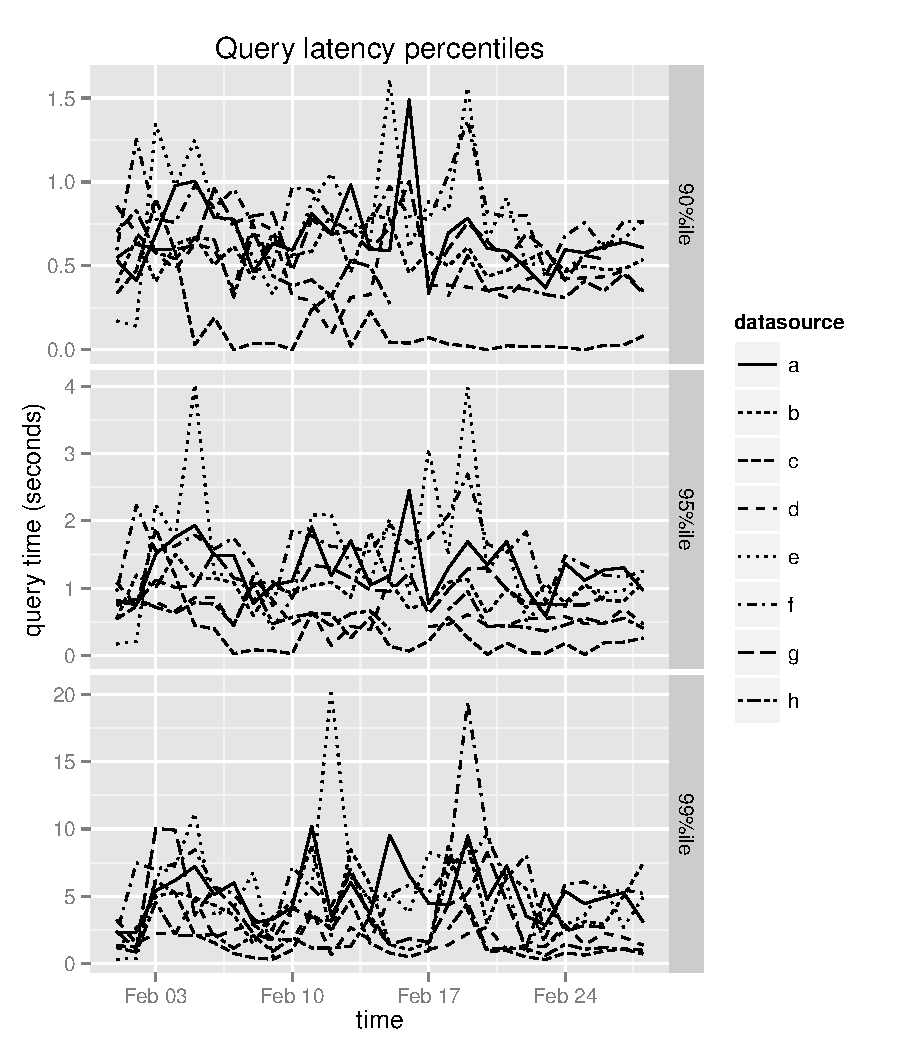
\includegraphics[width = 2.3in]{query_percentiles}
\caption{Query latencies of production data sources.}
\label{fig:query_latency}
\end{figure}

\begin{figure}
\centering
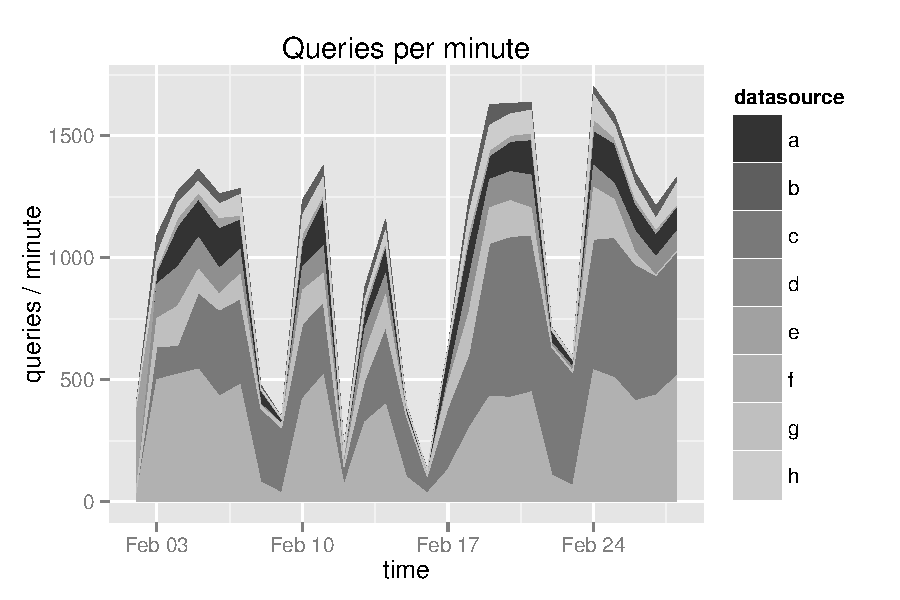
\includegraphics[width = 2.8in]{queries_per_min}
\caption{Queries per minute of production data sources.}
\label{fig:queries_per_min}
\end{figure}

\subsection{Query Benchmarks on TPC-H Data}
We also present Druid benchmarks on TPC-H data.
Most TPC-H queries do not directly apply to Druid, so we
selected queries more typical of Druid's workload to demonstrate query performance. As a
comparison, we also provide the results of the same queries using MySQL using the
MyISAM engine (InnoDB was slower in our experiments).

We selected MySQL to benchmark
against because of its universal popularity. We chose not to select another
open source column store because we were not confident we could correctly tune
it for optimal performance.

Our Druid setup used Amazon EC2
\texttt{m3.2xlarge} instance types (Intel\textsuperscript{\textregistered} Xeon\textsuperscript{\textregistered} E5-2680 v2 @ 2.80GHz) for
historical nodes and \texttt{c3.2xlarge} instances (Intel\textsuperscript{\textregistered} Xeon\textsuperscript{\textregistered} E5-2670 v2 @ 2.50GHz) for broker
nodes. Our MySQL setup was an Amazon RDS instance that ran on the same \texttt{m3.2xlarge} instance type.

The results for the 1 GB TPC-H data set are shown
in Figure~\ref{fig:tpch_1gb} and the results of the 100 GB data set are shown
in Figure~\ref{fig:tpch_100gb}. We benchmarked Druid's scan rate at
53,539,211 rows/second/core for \texttt{select count(*)} equivalent query over a given time interval
and 36,246,530 rows/second/core for a \texttt{select sum(float)} type query.

\begin{figure}
\centering
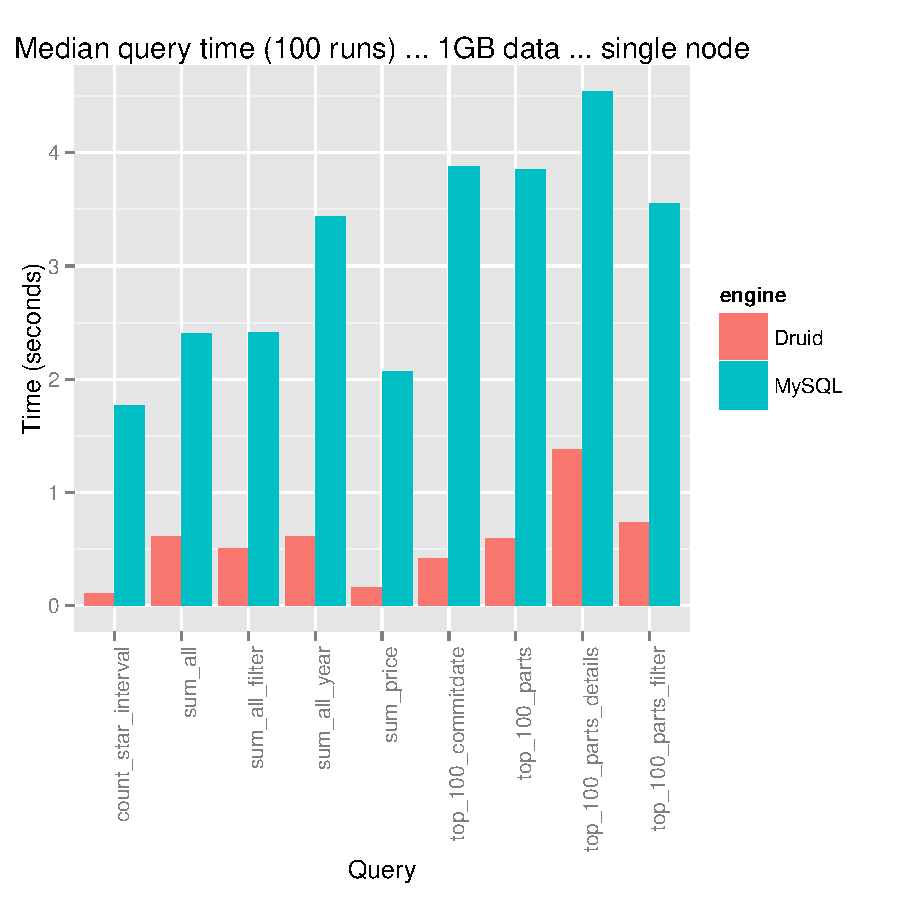
\includegraphics[width = 2.3in]{tpch_1gb}
\caption{Druid \& MySQL benchmarks -- 1GB TPC-H data.}
\label{fig:tpch_1gb}
\end{figure}

\begin{figure}
\centering
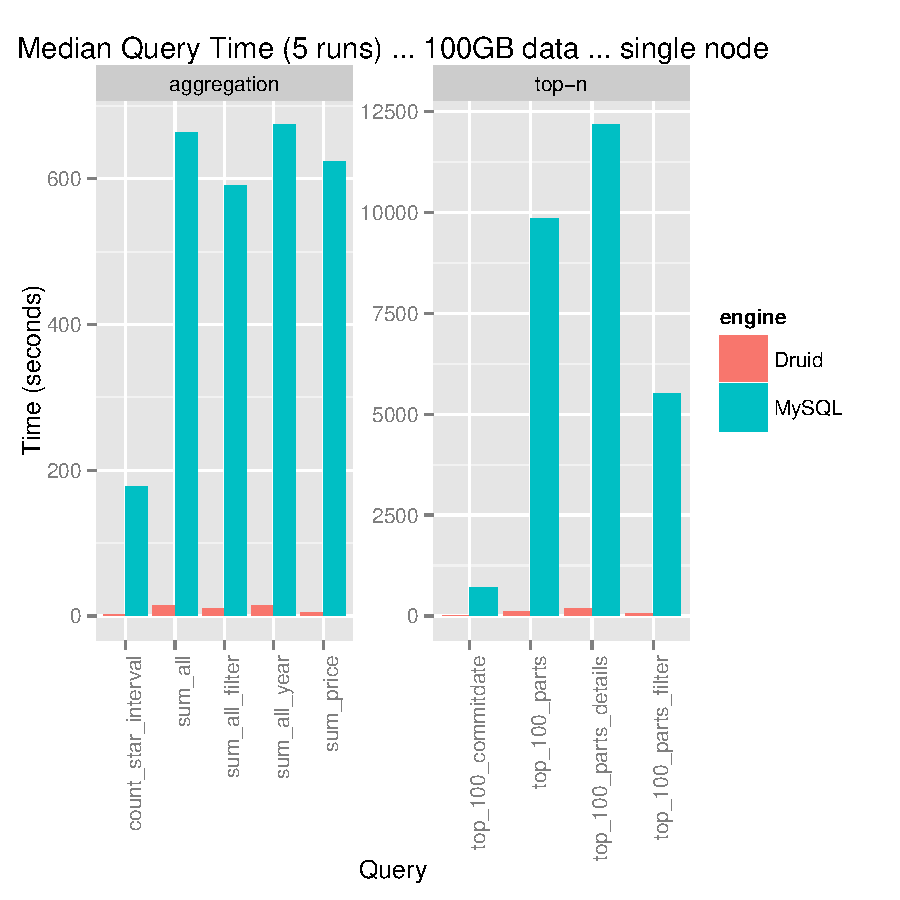
\includegraphics[width = 2.3in]{tpch_100gb}
\caption{Druid \& MySQL benchmarks -- 100GB TPC-H data.}
\label{fig:tpch_100gb}
\end{figure}

Finally, we present our results of scaling Druid to meet increasing data
volumes with the TPC-H 100 GB data set. We observe that when we
increased the number of cores from 8 to 48, not all types of queries
achieve linear scaling, but the simpler aggregation queries do,
as shown in Figure~\ref{fig:tpch_scaling}.

The increase in speed of a parallel computing system is often limited by the
time needed for the sequential operations of the system. In this case, queries
requiring a substantial amount of work at the broker level do not parallelize as
well.

\begin{figure}
\centering
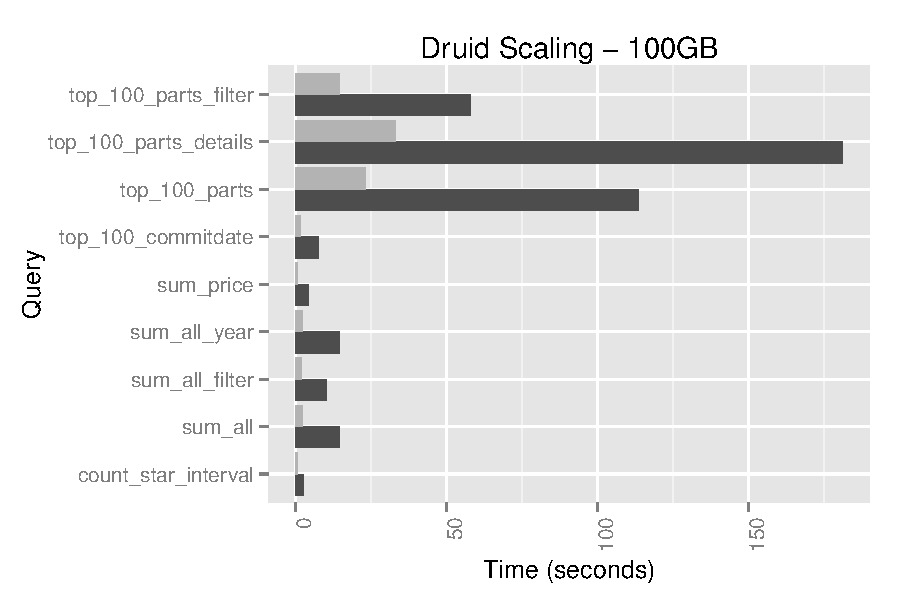
\includegraphics[width = 2.3in]{tpch_scaling}
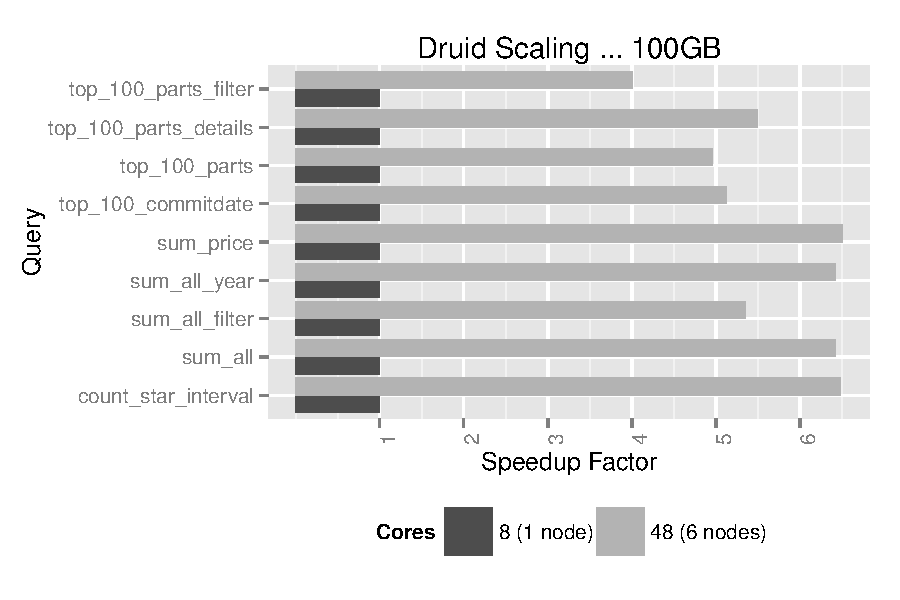
\includegraphics[width = 2.3in]{tpch_scaling_factor}
\caption{Druid scaling benchmarks -- 100GB TPC-H data.}
\label{fig:tpch_scaling}
\end{figure}

\subsection{Data Ingestion Performance}
To showcase Druid's data ingestion latency, we selected several production
datasources of varying dimensions, metrics, and event volumes. Our production
ingestion setup consists of 6 nodes, totalling 360GB of RAM and 96 cores
(12 x Intel\textsuperscript\textregistered Xeon\textsuperscript\textregistered E5-2670).

Note that in this setup, several other data sources were being ingested and
many other Druid related ingestion tasks were running concurrently on the machines.

Druid's data ingestion latency is heavily dependent on the complexity of the
data set being ingested. The data complexity is determined by the number of
dimensions in each event, the number of metrics in each event, and the types of
aggregations we want to perform on those metrics. With the most basic data set
(one that only has a timestamp column), our setup can ingest data at a rate of
800,000 events/second/core, which is really just a measurement of how fast we can
deserialize events. Real world data sets are never this simple.
Table~\ref{tab:ingest_datasources} shows a selection of data sources and their
characteristics.

\begin{table}
  \centering
  \begin{tabular}{| l | l | l | l |}
    \hline
    \scriptsize\textbf{Data Source} & \scriptsize\textbf{Dimensions} & \scriptsize\textbf{Metrics} & \scriptsize\textbf{Peak events/s} \\ \hline
    \texttt{s} & 7 & 2 & 28334.60 \\ \hline
    \texttt{t} & 10 & 7 & 68808.70 \\ \hline
    \texttt{u} & 5 & 1 & 49933.93 \\ \hline
    \texttt{v} & 30 & 10 & 22240.45 \\ \hline
    \texttt{w} & 35 & 14 & 135763.17 \\ \hline
    \texttt{x} & 28 & 6 & 46525.85 \\ \hline
    \texttt{y} & 33 & 24 & 162462.41 \\ \hline
    \texttt{z} & 33 & 24 & 95747.74 \\ \hline
  \end{tabular}
  \caption{Ingestion characteristics of various data sources.}
  \label{tab:ingest_datasources}
\end{table}

We can see that, based on the descriptions in
Table~\ref{tab:ingest_datasources}, latencies vary significantly and the
ingestion latency is not always a factor of the number of dimensions and
metrics. We see some lower latencies on simple data sets because that was the
rate that the data producer was delivering data. The results are shown in
Figure~\ref{fig:ingestion_rate}.

We define throughput as the number of events a
real-time node can ingest and also make queryable. If too many events are sent
to the real-time node, those events are blocked until the real-time node has
capacity to accept them. The peak ingestion latency we measured in production
was 22914.43 events/second/core on a datasource with 30 dimensions and 19 metrics,
running an Amazon \texttt{cc2.8xlarge} instance.

\begin{figure}
\centering
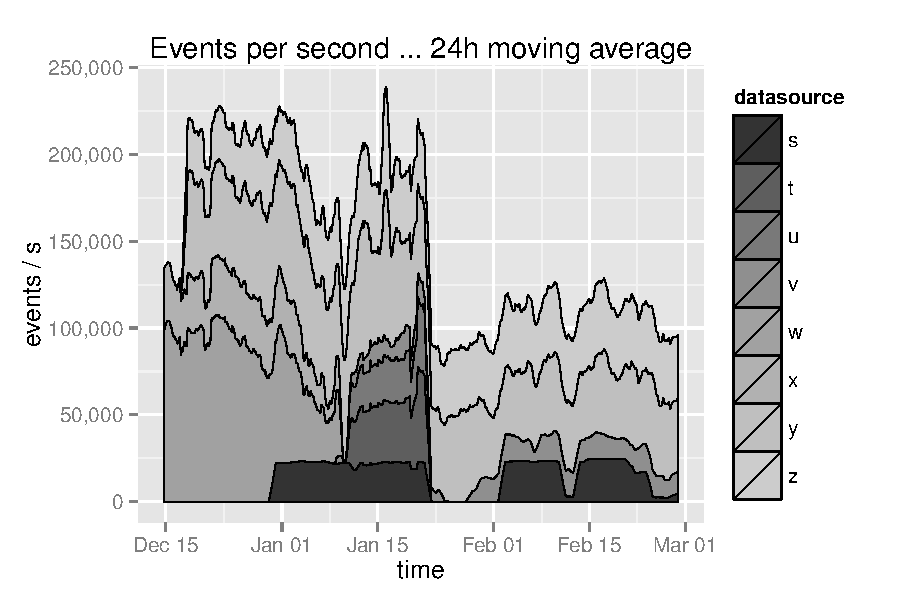
\includegraphics[width = 2.8in]{ingestion_rate}
\caption{Combined cluster ingestion rates.}
\label{fig:ingestion_rate}
\end{figure}

The latency measurements we presented are sufficient to address the stated
problems of interactivity. We would prefer the variability in the latencies to
be less. It is still possible to decrease latencies by adding
additional hardware, but we have not chosen to do so because infrastructure
costs are still a consideration for us.

\section{Druid in Production}\label{sec:production}
Over the last few years, we have gained tremendous knowledge about handling
production workloads with Druid and have made a couple of interesting observations.

\paragraph{Query Patterns}
Druid is often used to explore data and generate reports on data. In the
explore use case, the number of queries issued by a single user are much higher
than in the reporting use case. Exploratory queries often involve progressively
adding filters for the same time range to narrow down results. Users tend to
explore short time intervals of recent data. In the generate report use case,
users query for much longer data intervals, but those queries are generally few
and pre-determined.

\paragraph{Multitenancy}
Expensive concurrent queries can be problematic in a multitenant
environment. Queries for large data sources may end up hitting every historical
node in a cluster and consume all cluster resources. Smaller, cheaper queries
may be blocked from executing in such cases. We introduced query prioritization
to address these issues. Each historical node is able to prioritize which
segments it needs to scan. Proper query planning is critical for production
workloads. Thankfully, queries for a significant amount of data tend to be for
reporting use cases and can be deprioritized. Users do not expect the same level of
interactivity in this use case as when they are exploring data.

\paragraph{Node failures}
Single node failures are common in distributed environments, but many nodes
failing at once are not. If historical nodes completely fail and do not
recover, their segments need to be reassigned, which means we need excess cluster
capacity to load this data. The amount of additional capacity to have at any
time contributes to the cost of running a cluster. From our experiences, it is
extremely rare to see more than 2 nodes completely fail at once and hence, we
leave enough capacity in our cluster to completely reassign the data from 2
historical nodes.

\paragraph{Data Center Outages}
Complete cluster failures are possible, but extremely rare. If Druid is
only deployed in a single data center, it is possible for the entire data
center to fail. In such cases, new machines need to be provisioned. As long as
deep storage is still available, cluster recovery time is network bound, as
historical nodes simply need to redownload every segment from deep storage. We
have experienced such failures in the past, and the recovery time was
several hours in the Amazon AWS ecosystem for several terabytes of data.

\subsection{Operational Monitoring}
Proper monitoring is critical to run a large scale distributed cluster.
Each Druid node is designed to periodically emit a set of operational metrics.
These metrics may include system level data such as CPU usage, available
memory, and disk capacity, JVM statistics such as garbage collection time, and
heap usage, or node specific metrics such as segment scan time, cache
hit rates, and data ingestion latencies. Druid also emits per query metrics.

We emit metrics from a production Druid cluster and load them into a dedicated
metrics Druid cluster. The metrics Druid cluster is used to explore the
performance and stability of the production cluster. This dedicated metrics
cluster has allowed us to find numerous production problems, such as gradual
query speed degregations, less than optimally tuned hardware, and various other
system bottlenecks. We also use a metrics cluster to analyze what queries are
made in production and what aspects of the data users are most interested in.

\subsection{Pairing Druid with a Stream Processor}
Currently, Druid can only understand fully denormalized data
streams. In order to provide full business logic in production, Druid can be
paired with a stream processor such as Apache Storm \cite{marz2013storm}.

A Storm topology consumes events from a data stream, retains only those that are
“on-time”, and applies any relevant business logic. This could range from
simple transformations, such as id to name lookups, to complex operations
such as multi-stream joins. The Storm topology forwards the processed event
stream to Druid in real-time. Storm handles the streaming data processing work,
and Druid is used for responding to queries for both real-time and
historical data.

\subsection{Multiple Data Center Distribution}
Large scale production outages may not only affect single nodes, but entire
data centers as well. The tier configuration in Druid coordinator nodes allow
for segments to be replicated across multiple tiers. Hence, segments can be
exactly replicated across historical nodes in multiple data centers.
Similarily, query preference can be assigned to different tiers. It is possible
to have nodes in one data center act as a primary cluster (and receive all
queries) and have a redundant cluster in another data center. Such a setup may
be desired if one data center is situated much closer to users.

\section{Related Work}
\label{sec:related}
Cattell \cite{cattell2011scalable} maintains a great summary about existing
Scalable SQL and NoSQL data stores. Hu \cite{hu2011stream} contributed another
great summary for streaming databases. Druid, feature-wise, sits somewhere
between Google’s Dremel \cite{melnik2010dremel} and PowerDrill
\cite{hall2012processing}. Druid has most of the features implemented in Dremel
(Dremel handles arbitrary nested data structures while Druid only allows for a
single level of array-based nesting) and many of the interesting compression
algorithms mentioned in PowerDrill.

Although Druid builds on many of the same principles as other distributed
columnar data stores \cite{fink2012distributed}, many of these data stores are
designed to be more generic key-value stores \cite{lakshman2010cassandra} and do not
support computation directly in the storage layer. There are also other data
stores designed for some of the same data warehousing issues that Druid
is meant to solve. These systems include in-memory databases such as
SAP’s HANA \cite{farber2012sap} and VoltDB \cite{voltdb2010voltdb}. These data
stores lack Druid's low latency ingestion characteristics. Druid also has
native analytical features baked in, similar to ParAccel \cite{paraccel2013}, however,
Druid allows system wide rolling software updates with no downtime.

Druid is similiar to C-Store \cite{stonebraker2005c} and LazyBase \cite{cipar2012lazybase} in that it has
two subsystems, a read-optimized subsystem in the historical nodes and a
write-optimized subsystem in the real-time nodes. Real-time nodes are designed to
ingest a high volume of append heavy data, and do not support data updates.
Unlike the two aforementioned systems, Druid is meant for OLAP transactions and
not OLTP transactions.

Druid's low latency data ingestion features share some similarities with
Trident/Storm \cite{marz2013storm} and Spark Streaming
\cite{zaharia2012discretized}, however, both systems are focused on stream
processing whereas Druid is focused on ingestion and aggregation. Stream
processors are great complements to Druid as a means of pre-processing the data
before the data enters Druid.

There are a class of systems that specialize in queries on top of cluster
computing frameworks. Shark \cite{engle2012shark} is such a system for queries
on top of Spark, and Cloudera's Impala \cite{cloudera2013} is another system
focused on optimizing query performance on top of HDFS. Druid historical nodes
download data locally and only work with native Druid indexes. We believe this
setup allows for faster query latencies.

Druid leverages a unique combination of algorithms in its
architecture. Although we believe no other data store has the same set
of functionality as Druid, some of Druid’s optimization techniques such as using
inverted indices to perform fast filters are also used in other data
stores \cite{macnicol2004sybase}.

\section{Conclusions}
\label{sec:conclusions}
In this paper we presented Druid, a distributed, column-oriented, real-time
analytical data store. Druid is designed to power high performance applications
and is optimized for low query latencies. Druid supports streaming data
ingestion and is fault-tolerant. We discussed Druid benchmarks and
summarized key architecture aspects such
as the storage format, query language, and general execution.

\balance

\section{Acknowledgements}
\label{sec:acknowledgements}
Druid could not have been built without the help of many great engineers at
Metamarkets and in the community. We want to thank everyone that has
contributed to the Druid codebase for their invaluable support.

% The following two commands are all you need in the
% initial runs of your .tex file to
% produce the bibliography for the citations in your paper.
\bibliographystyle{abbrv}
\bibliography{druid}  % druid.bib is the name of the Bibliography in this case
% You must have a proper ".bib" file
%  and remember to run:
% latex bibtex latex latex
% to resolve all references

%Generated by bibtex from your ~.bib file. Run latex,
%then bibtex, then latex twice (to resolve references).

%APPENDIX is optional.
% ****************** APPENDIX **************************************
% Example of an appendix; typically would start on a new page
%pagebreak

\end{document}
